\documentclass[12pt]{IEEEtran}

%\hyphenation{}
\usepackage{cite}
\usepackage{graphicx}
\usepackage{hyperref}
\usepackage{amsmath, amsfonts}
\usepackage{url}
\usepackage{subcaption}
\usepackage[ruled,vlined,commentsnumbered,titlenotnumbered,norelsize]{algorithm2e}

% Line break with additional spacing. Default is .75 line-height extra spacing
% Extra space is put in to allow line breaks immediately after \item
\newcommand{\br}[1][.75]{\ \\[#1\baselineskip]}

\renewcommand\thesection{\arabic{section}}
\renewcommand\thesubsection{\thesection.\arabic{subsection}}
\renewcommand\thesubsubsection{\thesubsection.\arabic{subsubsection}}

\renewcommand\thesectiondis{\arabic{section}}
\renewcommand\thesubsectiondis{\thesectiondis.\arabic{subsection}}
\renewcommand\thesubsubsectiondis{\thesubsectiondis.\arabic{subsubsection}}

\begin{document}

\title{Training a Pok\'{e}mon Puzzle League Champion}
\author{Logan~Short, Christopher~Wong}% <-This % stops a space
\markboth{CS 221 Final Project, Autumn 2015}{}
\maketitle

\begin{abstract}
Due to their strict state based nature, puzzle games have always served as ideal problems for the exploration and progression of artificial intelligence methodology. In this paper, we explore the development of a computer vision based AI agent for the video based puzzle game, Pok\'{e}mon Puzzle League.
\end{abstract}

\section{Introduction}
\IEEEPARstart{P}{ok\'{e}mon} Puzzle League is a puzzle game released by Nintendo in September 2000 for the Nintendo 64 entertainment system. In this paper, we discuss our development of an AI agent that can play the game at a high level. We begin by briefly summarizing previous relevant work in the puzzle game and computer vision areas. Next, we give an overview of general game play and strategy. We then discuss the implementation details of our end-to-end system, which includes two major components: (1) extracting and modeling game state, and (2) computing the best short-term sequence of moves to maximize the agent's in-game advantage. Finally, we conclude with our results and an analysis of the strengths and weaknesses of our approach.

\begin{figure}[h!]
\centerline{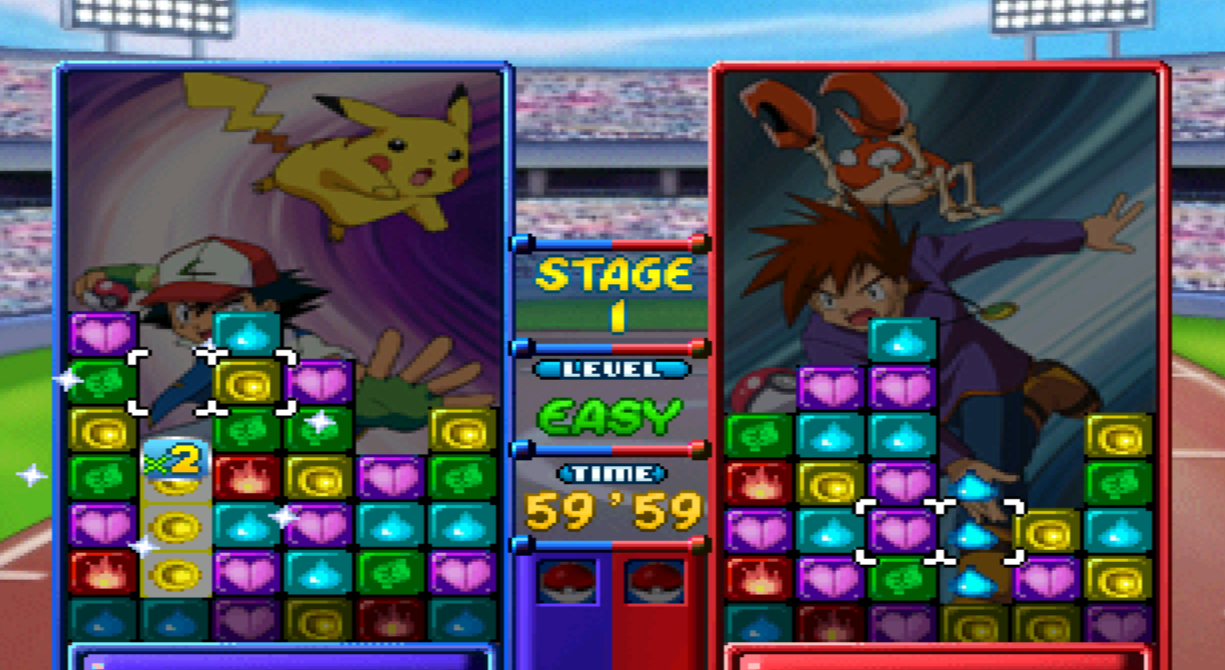
\includegraphics[width=3.4in]{game.png}}
\caption{Screenshot of $2$-player ``Versus'' gameplay.}
\label{fig:game}
\end{figure}

\section{Related Work}
Although we were not able to find many previous research papers relevant to our topic, we still obtained a few which were influential in our design. Here, we summarize two of the most significant pieces.

\subsection{\href{https://http://cns-classes.bu.edu/cn550/Readings/frey-slate-91.pdf}{Letter Recognition using Holland-Style Adaptive Classifiers} (Frey and Slate, 1991)}
In \cite{1}, Frey and Slate utilize an adaptive classifier to successfully recognize letters from images. The classifier implemented by the paper constructs $16$-dimensional feature vectors that can be used to represent images with features being selected to represent certain characteristics that different letters in the English alphabet might possess. An example feature included the density of ``on'' (present) pixels below the horizontal middle of the letter image. A dataset consisting of character images from $20$ different fonts with slight alterations, such as scaling or rotation, was then used to train the classifier. Frey and Slate found that, by utilizing this approach, they were able to achieve high levels of accuracy for English letter prediction.

\subsection{\href{https://hal.inria.fr/inria-00418954/document}{Building Controllers for Tetris} (Thiery and Scherrer, 2009)}
In \cite{2}, Thiery and Scherrer provide an overview of the three most successful methods for automated playing of the video game Tetris. The first two, hand-written evaluation and general purpose optimization both attempt to optimize weights for features that represent the quality of a move. These two methods are noted to have achieved the most success in Tetris gameplay. Reinforcement learning attempts to learn a policy for achieving an optimal expected future score. Thiery and Scherrer point out that Tetris might be too complicated of a game for state-of-the-art reinforcement learning approaches; thus these methods have not been as successful. Based on the results of this paper, we decided to avoid a reinforcement learning based approach for our AI system and instead focused on other avenues such as randomized algorithms.

\section{Gameplay and Task Definition}

We being by giving a brief overview of the game and the goals of our AI agent. In Section $3.1$, we explain general gameplay mechanics, while in Section $3.2$, we formally define the task at hand. In Section $3.3$, we give initial benchmark results of our oracle and baseline implementation.

\subsection{Gameplay}
Pok\'{e}mon Puzzle League is played on a grid-based board 6 tiles wide and 12 tiles tall. Each space in the board can be occupied by a block, which can be one of several types. Players control a freely moving cursor that encapsulates two horizontally adjacent grid squares. At any time, the player can choose to swap the positions of the two blocks currently selected by the cursor. If there ever exists a series of three or more blocks of the same type in a line, these blocks are cleared from the board. New blocks will slowly appear from the bottom, causing the entire grid to continuously rise to the top. If the blocks reach the top, the player loses.

There are $1$-player and $2$-player modes for the game. In the $1$-player ``Endless'' mode, the human player plays for as long as possible, attempting to get the highest score before losing. In the $2$-player ``Versus'' mode, clearing many blocks quickly causes garbage blocks to be sent to the opponent's board. To destroy garbage blocks, one can make a $3$-in-a-row (or larger) adjacent to a garbage block. This will deconstruct the garbage block into random normal blocks, thus allowing them to be cleared normally. The goal in this mode is to outlast one's opponent. Figure~\ref{fig:game} is a screenshot of gameplay in ``Versus'' mode.

In either mode, it is beneficial for a player to create combos and chains. In the $1$-player mode, a player will receive more points, and in the $2$-player mode, the player will send larger garbage blocks to the opponent. Combos are created when there are more than $3$ blocks cleared at one time. A chain is created when, after a clear, blocks fall to create additional clears. Figure~\ref{fig:chain} demonstrates a simple chain taking place. Chains are more valuable than combos.

\begin{figure}[h!]
\centerline{\begin{subfigure}[h]{1.3in}
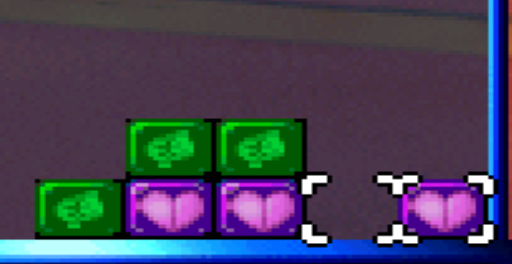
\includegraphics[width=1.3in]{chain1.png}
\end{subfigure}}\br[.5]
\centerline{$\Downarrow$}\br[.5]
\centerline{\begin{subfigure}[h]{1.3in}

\includegraphics[width=1.3in]{chain2.png}
\end{subfigure}}\br[.5]
\centerline{$\Downarrow$}\br[.5]
\centerline{\begin{subfigure}[h]{1.3in}

\includegraphics[width=1.3in]{chain3.png}
\end{subfigure}}
\caption{Clearing a simple $2$x chain.}
\label{fig:chain}
\end{figure}

\subsection{Task Definition}

The goal of our system is to produce an automated agent that is capable of playing Pok\'{e}mon Puzzle League at a high level. We noticed that the two modes of the game are a lot more similar than they are different. In each case, the player wants to create large combos and long chains, while preventing his or her grid from reaching the top. With this in mind, we claim that optimal game strategy is largely the same in both modes, and so it is feasible to consider both cases at the same time. We will attempt to maximize our score in ``Endless'' mode and beat the in-game CPU consistently in ``Versus'' mode. We note that the in-game CPU can play at various difficulties, allowing us to record results at multiple levels.

\subsection{Oracle and Baseline}

We now give a few benchmark results. Using the game interface infrastructure explained in Sections $4$ and $5$, we quickly implemented a random AI agent which made $5$ random moves per second. This served as our baseline, and we fully expected all of our advanced algorithms (discussed in Section $6$) to beat it. For an oracle, we played the game ourselves, since we were the best game players we could find, human or machine.

Table~\ref{tab:baseline} records the performance for our baseline and oracle in $2$-player mode. We played against the in-game CPU at each level a total of $20$ times and recorded how many wins each method produced. There are five levels: Easy (E), Medium (M), Hard (H), Very Hard (VH), and Super Hard (SH). Since the game is rather complicated, the baseline AI does not do very well.

\begin{table}[ht]
\begin{center}
\begin{tabular}{c||c|c|c|c|c}
Difficulty & E & M & H & VH & SH \\ \hline\hline
Baseline & $5$ & $2$ & $0$ & $0$ & $0$ \\ \hline
Oracle & $20$ & $20$ & $19$ & $13$ & $3$
\end{tabular}
\end{center}
\caption{Baseline and oracle performance for $2$-player mode.}
\label{tab:baseline}
\end{table}

To complete our benchmark results, we also played the $1$-player mode $5$ times with each method, recording the average score achieved. Our baseline yielded an average score of $2460$, while our oracle was able to score much higher at $18781$.

\section{Approach}

Before delving into technical details, we give a high-level overview of our end-to-end system.

\subsection{System Overview}

When playing the game, we did not have access to the game's internal workings, memory, or data, so we could only rely on what was being displayed on screen. So, our first step involved building out an interface to the game. We emulated the game using the popular Dolphin Emulator. The Dolphin Emulator was ideal for our system because it offered two important features: (1) a native way to capture in-game screenshots, and (2) a native way to send movement inputs to the game at a quick rate. This ensured stability was much preferred over relying on external methods such as third-party applications to take screenshots or system calls to generate unreliably interpreted keyboard events. In particular, for movement input, Dolphin exposes an interface for named pipe communication.

With the interface in hand, we broke our problem down into a straightforward sequence of steps, which were to be looped until the game ended:
\begin{enumerate}
\item Capture an in-game screenshot.
\item Check if the game has ended. If so, stop.
\item Extract the agent's grid from the screenshot.
\item Calculate the best short sequence of moves possible on the grid.
\item Send the sequence of moves to the game.
\end{enumerate}
For performance reasons, it was infeasible to capture and parse a screenshot before each individual move. To compromise, we decided that calculating and executing a short sequence of $5$ to $10$ moves would still yield comparable results.

\subsection{Game State Model}

When parsing a game screenshot, it is straightforward for us to represent the board state internally as a grid that is $6$ blocks wide and $12$ blocks tall. There are a finite number of block types -- including garbage blocks and empty space -- so we can enumerate all possible values that a grid cell can take. Our model can deterministically calculate future board states after a series of moves by considering switches, clears, and falling blocks.

\section{Board Detection}

The first major component of our system required the ability to read the state of our agent's board from a screenshot of the game. This involved applying various techniques and heuristics learned from classification problems and computer vision. Image manipulation was done with the help of OpenCV. We discuss the general grid extraction in Section $5.1$, and we describe the specific details of classifying grid blocks in Section $5.2$.

\subsection{Grid Extraction}

Given a screenshot, we first isolated the agent's board, as shown in the first picture of Figure~\ref{fig:filter}. Next, before considering any sort of grid overlay, we removed the static game background from behind the board. Motivations for this will be discussed in Section $5.2$. To do so, we manually acquired the background image without any blocks. Then, with our target image, we compared each pixel to the background image, and set to black any locations which had an exact RGB match. This process was very accurate; an example output is seen in the second picture of Figure~\ref{fig:filter}.

\begin{figure}[h!]
\centerline{\begin{subfigure}[h]{1.5in}
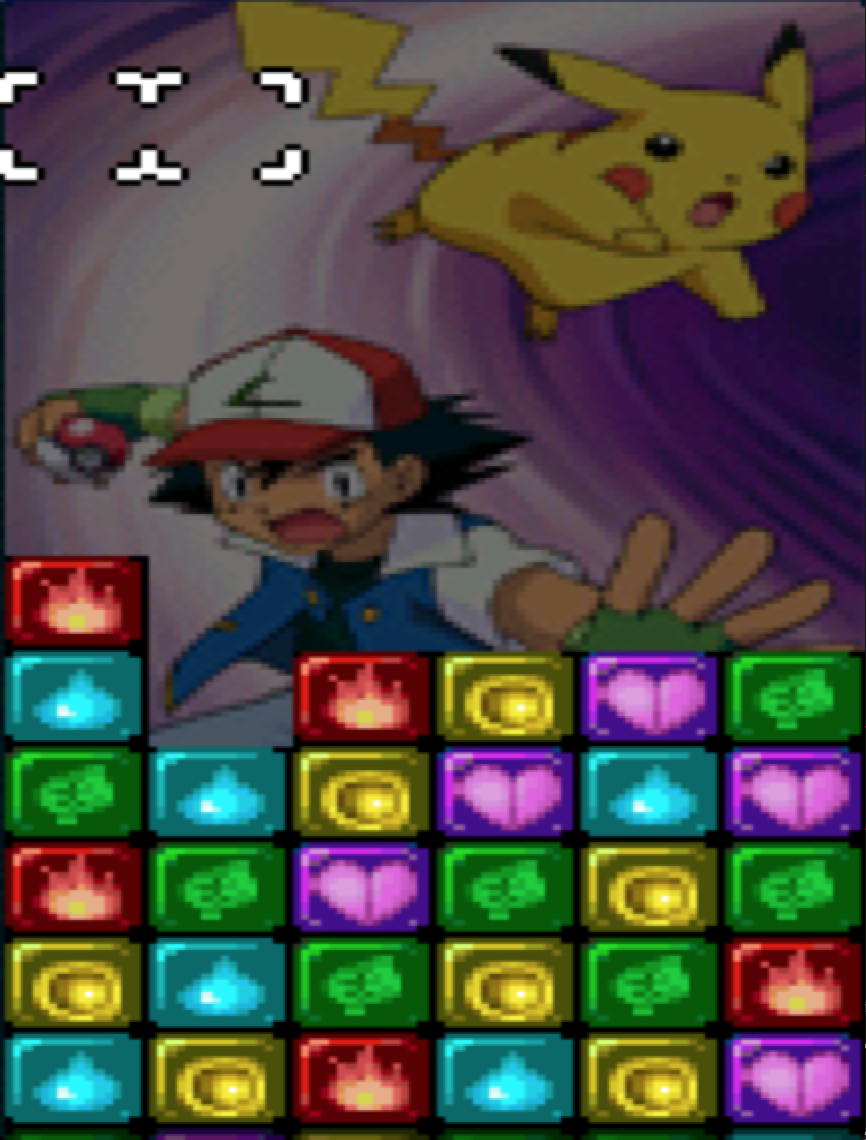
\includegraphics[width=1.5in]{filter1.png}
\end{subfigure}
~~
\begin{subfigure}[h]{1.5in}
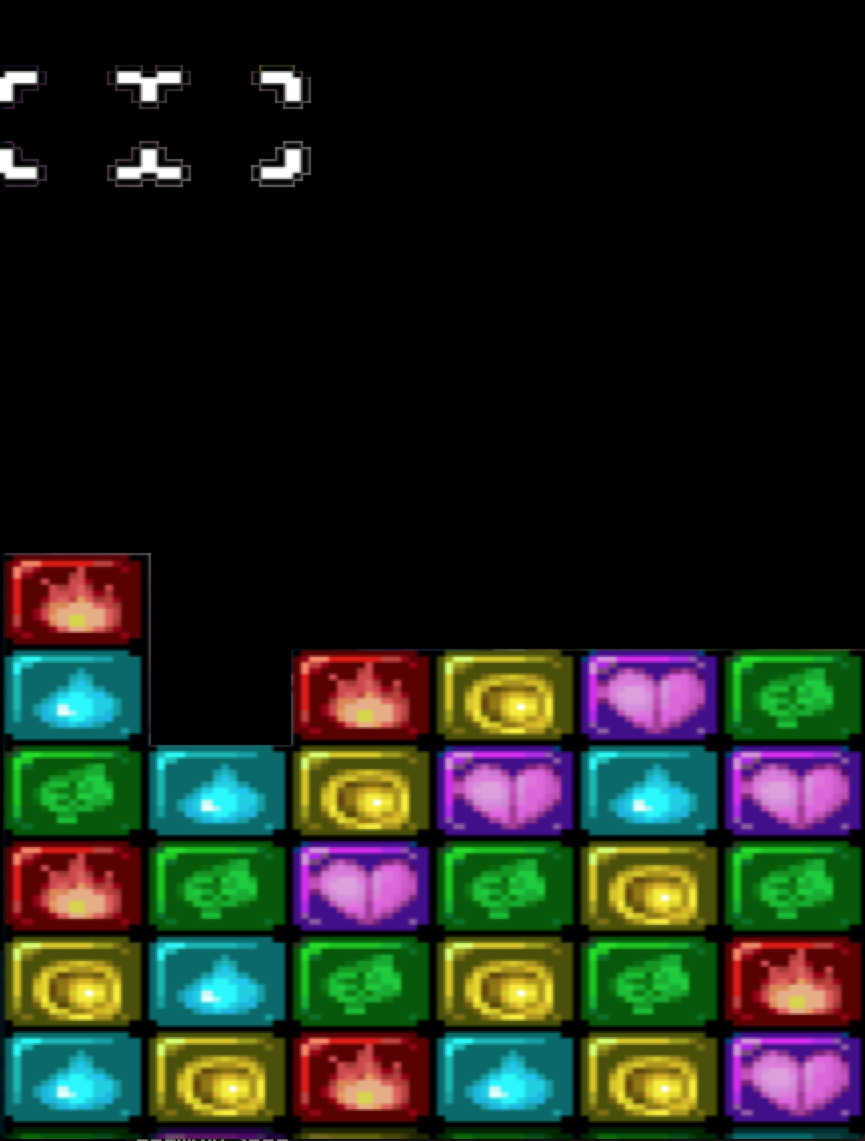
\includegraphics[width=1.5in]{filter2.png}
\end{subfigure}}
\caption{Side-by-side comparison of a grid before and after its background has been filtered out.}
\label{fig:filter}
\end{figure}

The next challenge was to determine the position of the grid within the image. As discussed in Section $3.1$, the locations of the blocks are not static; over time, the blocks slowly rise to the top as new blocks are introduced at the bottom. So, even though the dimensions of each blocks are consistent, the ``offset'' of the grid is variable. To solve this, we considered the simpler problem of trying to find the first row. Armed with our classifier $C$ (discussed in Section $5.2$) that outputs both predictions and prediction probabilities, we considered the likelihood of the first row image $R$ produced by a particular offset $y$. Whichever offset $y^*$ yielded the greatest likelihood was our answer. To calculate the likelihood for $y$ and its corresponding row image $R$, we split $R$ into the appropriate blocks and classified them. Each classification has a probability score associated with it, and we multiplied these together.

Let $T$ be all possible block types, $f_C(t, b)$ be $C$'s classification probability that block $b$ is type $t$, and $H$ be the standard block height. Then, our grid offset calculation is concisely written as
\[ y^* := \arg\max_{0 \leq y < H} \sum_{b \in R} \max_{t \in T} f_C(t, b). \]

After determining $y^*$, splitting the grid is straightforward. Figure~\ref{fig:grid} shows a successful grid overlay. Note the nontrivial grid offset.

\begin{figure}[h!]
\centerline{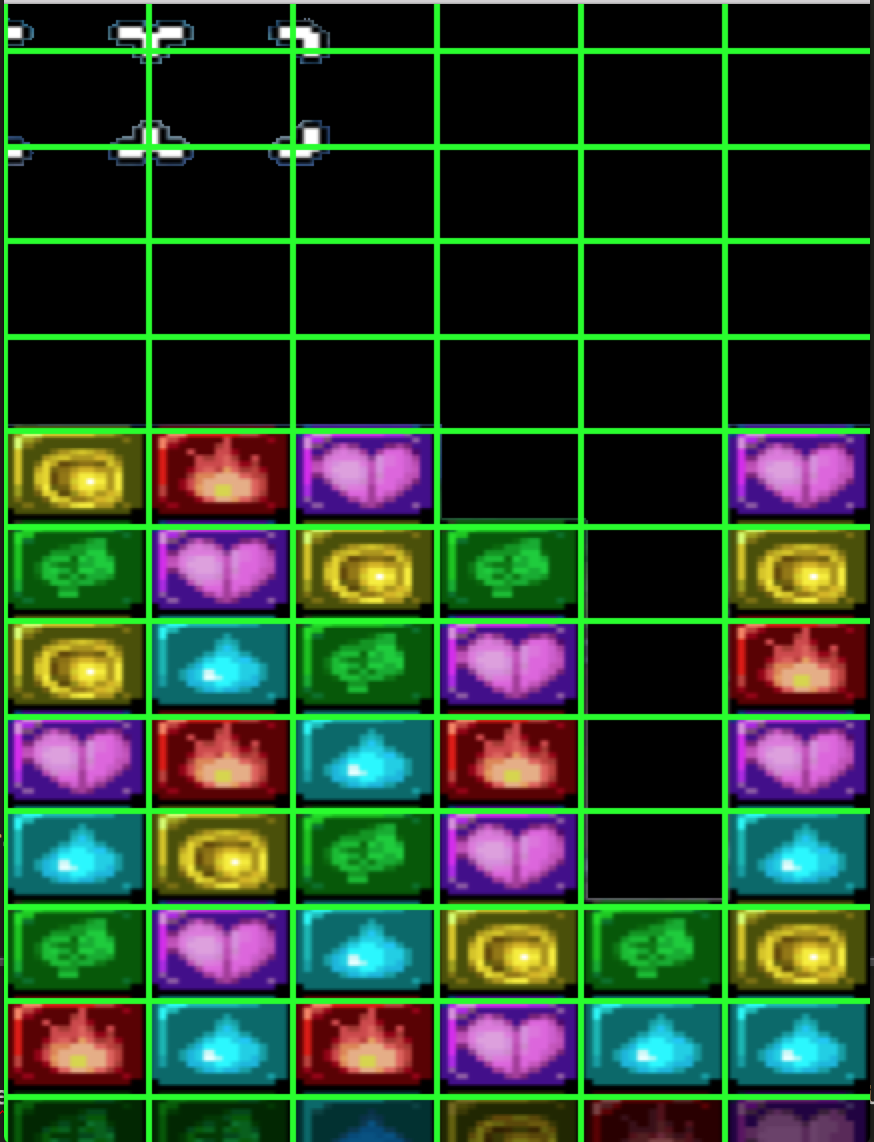
\includegraphics[width=1.5in]{grid.png}}
\caption{Dividing the board into a grid.}
\label{fig:grid}
\end{figure}

\subsection{Block Classification}

We trained and used a logistic regression classifier to predict the type of each block. One of the benefits this offered us was that, in addition to providing a prediction, it also gave the probability (score) of the prediction itself. This was useful for our methods just discussed in Section $5.1$. We also experimented with using a classifier based on $k$-NN -- with inverse distances being the score -- but it eventually yielded slightly worse prediction accuracy.

One of the main focuses for this classification problem was determining the optimal feature vector for a given block $b$. For our first attempt, we simply used the raw pixel RGB values as one long, flattened feature vector. At our image resolution, this meant that $\phi(b) \in \mathbb{R}^{10152}$. This was quite a large number of dimensions, but we reasoned that, since a block type never changes in appearance, it could still be accurate.

This method, however, turned out to be unreliable. The slightest noise severely impacted our classification accuracy, such as the grid offset $y^*$ being even $1$ or $2$ pixels off. Since our overall system had tight performance requirements, we could not afford the time to stabilize the noise to match feature vectors. Thus, inspired by \cite{1}, we decided to use more descriptive features. We separated $b$ into its R, G, and B color channels, and for each channel, we calculated the mean, median, and standard deviation over all the pixels. We also noticed that the image ``noise'' usually concentrated at the edges of $b$, either due to the white cursor or thin black border. Thus, we cropped a $5$-pixel border around $b$ to obtain $b'$, and again we calculated the mean, median, and standard deviation for each color channel. In the end, we concatenated all of these features to yield $\phi(b) \in \mathbb{R}^{18}$. This was a much easier feature vector to work with, and it yielded the accurate performance that we needed, both in prediction accuracy and runtime within our classifier.

The properties of our new feature vector motivated us to filter the game background, as discussed in Section $5.1$. Since $\phi$ aggregates some statistics about the color of each square, we suffered from incorrect classifications if the background image at a particular square was close in color to an actual block type. For example, the yellow Pikachu character in the upper right corner (see Figure~\ref{fig:filter}) often produced a ``yellow'' classification before we filtered the background.

\section{Algorithms}

The second major component of our system involved designing and implementing the best algorithm possible to compute optimal move sequences. There are several properties we considered for our ideal algorithm:
(1) Since the game is played in real time, calculating an optimal set of moves must be able to return a strong set of moves relatively quickly. Consequently, producing decent moves in a short amount of time is preferable to an algorithm that returns very strong moves but requires a large amount of processing time.
(2) The board state only changes when a swap is made. Moving the cursor around the board does not affect the position of pieces in any way. Our algorithms can thus focus on optimal swaps, especially since the movement of the cursor is abstracted away by our game interface.
(3) High level gameplay revolves around setting up combos and chains that can be triggered by one swap. As such, it is better to attempt to find an optimal sequence of ``setup'' swaps that leads to one very influential swap, instead of trying to find optimal singleton swaps one at a time.

Given these considerations, we decided to explore two avenues of algorithms for determining optimal move sequences. The first of these is exhaustive tree search, discussed in Section $6.2$. This algorithm attempts to find an optimal move sequence by evaluating all possible move sequences up to a certain move length depth. It uses an evaluation function, described in Section $6.1$, to determine the utility of each move sequence. The second avenue lies in the space of randomized algorithms. These evaluate sequences using the same evaluation function, but the strength of these algorithms lies in their ability to quickly determine sequences of moves that yield relatively strong results. We implemented a standard Random Algorithm (Section $6.3$) and a Genetic Algorithm (Section $6.4$). This fits our needs well since it is not necessary that we perform an exhaustive search to find a board's true optimal sequence of moves.

\subsection{Evaluation Function}

The primary goal for our board evaluation function is to give high scores to boards that contain large combos and chains and give lower scores to boards that do not result in very many pieces being cleared. In addition, since chains yield better results than combos and longer chains are optimal, our evaluation function should favor long chains over large combos. We thus decided to go with a simple evaluation function that mapped this relationship directly by summing over the number of tiles cleared at each chain level, multiplied by the chain level. If we define $B$ to be a board, $S(B)$ to be the score of $B$, and $k_i$ to be the number of pieces matched and cleared at chain multiplier $i$ for the board $B$, our evaluation function is of the form:
\begin{align*}
S(B) = \sum_{i}i \cdot k_i
\end{align*}

In addition to maximizing the number of large combos and chains, an optimal strategy must also focus on keeping itself alive. The game ends in a loss if any of the board's columns stack up to the top row of the board. We thus added a component to our evaluation function that subtracts from the score based on the height of the board's columns after all combos and chains have been cleared from the board. Since only one column needs to become too high in order for the game to result in a loss, our evaluation function attempts to make sure no columns reach extreme heights by applying a negative weight proportional to the cube of each column's height. Defining $c$ to be an index over all the columns in the board and $H_c$ to be the height of column $c$, the final evaluation function is of the form:
\begin{align*}
S(B) = \sum_{i}i \cdot k_i - \sum_{c} \frac{1}{1000}H_c^3
\end{align*}
It should be noted that, when calculating the total score of a move sequence by summing over the scores of all intermediate boards, the negative weights associated with column heights should only be applied once at the end of the sequence.

\subsection{Exhaustive Search}
A basic approach to determining an optimal move sequence is to exhaustively examine all possible combinations of moves and evaluate the resulting board states. This process involves generating a tree in which the root of the tree is some initial board configuration and the $i$th level of the tree contains all boards reachable on the $i$th move of a move sequence. The successors of a board state $B$ can be found by applying all possible moves to $B$. The successors of all boards on a level $i$ then inhabit level $i+1$ of the tree. A move sequence is thus represented by a path along this tree, where each move in the sequence represents the edge taken to get to the next tree level. Since we are concerned with the overall quality of a move sequence, the score of a move sequence can be calculated as the sum of the scores of each of the board states located on the sequence's path. The sequence with the highest score can then be returned as the chosen combination of moves.

\begin{algorithm}\label{exhaustive}\small
\caption{\small Exhaustive$(B, numMoves)$}
$\alpha \gets 0$ \\
$\beta \gets $ empty list\\
$S \gets [ \ (B, 0) \ ]$ \\
\ForEach{$i \in $ range(0,numMoves)}{
$newS \gets [ \ ]$ \\
\ForEach{$B', s' \in S$}{
\ForEach{$move \in AllMoves$}{
$B' \gets$ Apply $move$ to $B'$ \\
$s' \gets s' + Evaluate(B')$ \\
append $(B', s')$ to $newS$ \\
}
}
$S \gets newS$\\
}
$\beta , \alpha \gets \max_{s'}(S)$ \\
return $\alpha, \beta$
\end{algorithm}

\subsection{Random Algorithm}

The first of our randomized approaches is a Random Algorithm that works by generating a series of sequences of random board position swaps. Each sequence is then applied to the board and the board evaluation scores after each swap are totaled as in the Exhaustive Search to obtain the final score of the move sequence. The sequence which yields the highest score is returned as the chosen move sequence. The variables for this algorithm are the number of randomly generated sequences to test and the number of swaps used in a sequence. Increasing the number of tested sequences tends to yield better results at the cost of runtime. Increasing the number of moves in a sequence tends to yield larger combos and chains but also increases the runtime.

\begin{algorithm}\label{random}\small
\caption{\small Random$(B, numTrials, numMoves)$}
$\alpha \gets 0$ \\
$\beta \gets $ empty list\\
\ForEach{$i \in $ range(0,numTrials)}{
$\alpha' \gets 0$ \\
$\beta' \gets$ generate random sequence of $numMoves$ swaps \\
\ForEach{$m \in \beta'$}{
$B \gets$ Apply $m$ to $B$ \\
$\alpha' \gets \alpha' + Evaluate(B)$
}
rollback $B$ \\
\If{$s > \alpha$}{
$\alpha \gets \alpha'$ \\
$\beta \gets \beta'$ \\
}
}
return $\alpha, \beta$
\end{algorithm}

\subsection{Genetic Algorithm}

Building upon the Random Algorithm, we decided to implement a Genetic Algorithm which attempts to combine the best parts of randomly generated move sequences in order to produce a more optimal sequence. Our Genetic Algorithm begins by generating a set of random swap sequences, $S$. Each of these move sequences is scored by summing the evaluation scores of the resulting board after each swap in the sequence. A new generation of sequences is then formed by selecting two sequences from $S$. During this selection process, the probability of selecting a sequence $a$ is based on the relative score of $a$ in comparison to all other sequences in $S$, with higher scores yielding higher probabilities. Once two sequences have been selected, a pivot index is picked uniformly at random. A child is generated by concatenating all the swaps up to the pivot index of one sequence with all the swaps after the pivot point of the other sequence. Thus this process generates two children. These children are added to a new sequence set $S'$ and the child generating process is continued until the size of $S'$ is equal to the size of $S$. We then set $S$ to be equal to $S'$ and repeat the process. After a specified number of generations, we return the move sequence in $S$ that yields the highest score.

Variables for this algorithm include the size of the set $S$, the number of generations to run, and the length of a move sequence. As with the Random Algorithm, increasing these parameters yields better results at the cost of increased runtime. An additional variable is the probability distribution of sequence selection based on the scores. Initial testing seems to indicate that having the selection probability be based on a distribution made up of the squares of sequence scores yields favorable results.

\begin{algorithm}\label{genetic}\small
\caption{\small Genetic$(B, numSeq, numGen, numMoves)$}
$S \gets$ list of $numSeq$ random sequences of $numMoves$ swaps\\
\ForEach{$i \in$ range(0,numGen)}{
$S' \gets$ empty list\\
$seq1 \gets$ pick from $S$ with probability based on Evaluate() score \\
$seq2 \gets$ pick from $S$ with probability based on Evaluate() score \\
$p \gets$ uniformly random value in $range(0,numMoves)$ \\
$child1 \gets seq1[0:p] + seq2[p:numMoves]$ \\
$child2 \gets seq2[0:p] + seq1[p:numMoves]$ \\
append $child1, child2$ to $S'$ \\
$S \gets S'$
}
return sequence in $S$ with best Evaluate() score\\
\end{algorithm}

\section{Results and Analysis}

Finally, in Section $7.1$, we give the results obtained by using our various algorithms. Sections $7.2$ and Sections $7.3$ follows this with an error analysis of the results, and why they can be explained by citing the strengths and weaknesses of each algorithm.

\subsection{Algorithm Results}

Table~\ref{tab:versus} records the performance of all of our algorithms in the $2$-player ``Versus'' mode. Like before, we played $20$ times against each level of the in-game CPU and recorded the number of wins. For convenience of comparison, we have included our baseline and oracle results as well.

\begin{table}[ht]
\begin{center}
\begin{tabular}{c||c|c|c|c|c}
Difficulty & E & M & H & VH & SH \\ \hline\hline
Baseline & $5$ & $1$ & $0$ & $0$ & $0$ \\ \hline
Exhaustive & $13$ & $4$ & $0$ & $0$ & $0$ \\ \hline
Random & $19$ & $15$ & $9$ & $2$ & $0$ \\ \hline
Genetic & $20$ & $17$ & $6$ & $0$ & $0$ \\ \hline
Oracle & $20$ & $20$ & $19$ & $13$ & $3$
\end{tabular}
\end{center}
\caption{Results for $2$-player mode.}
\label{tab:versus}
\end{table}

Next, Table~\ref{tab:endless} reports the average scores achieved by each of our algorithms in the $1$-player ``Endless'' mode. Each algorithm was tested $5$ times. Again, we include the baseline and oracle scores for convenience.

\begin{table}[ht]
\begin{center}
\begin{tabular}{c||c}
& Score \\ \hline\hline
Baseline & $1260$ \\ \hline
Exhaustive & $3020$ \\ \hline
Random & $6712$ \\ \hline
Genetic & $7126$ \\ \hline
Oracle & $18781$
\end{tabular}
\end{center}
\caption{Results for $1$-player mode.}
\label{tab:endless}
\end{table}

\subsection{Board Detection Error Analysis}

As discussed in Section $5$, we carefully implemented our grid detection process to be as robust as possible. That being said, we were still prone to two major errors, both of which had significant negative impacts on our performance.

The first error surfaced whenever the grid offset was not calculated appropriately. In this situation, the blocks would not be parsed correctly, and our AI algorithms would thus calculate garbage move sequences. This was damaging because it took valuable seconds to calculate and perform wasted moves. As the rising speed (in ``Endless'' mode) or the CPU speed (in ``Versus'' mode) got faster, an incorrect grid extraction could potentially reuslt in losing the entire game.

The second error was related to our classifier's difficulty to differentiate garbage blocks from similar looking actual blocks. Consider the appearance of a yellow garbage block, shown in Figure~\ref{fig:garbage}.
\begin{figure}[h!]
\centerline{
\includegraphics[width=1.5in]{garbage.png}}
\caption{Yellow garbage block.}
\label{fig:garbage}
\end{figure}
Recall that our feature vector $\phi$ aggregates color statistics in favor of pixel values. This yellow garbage block is too similar in color to the actual yellow block, so our classifier misclassifies the entire thing. This is also severely damaging for our AI algorithms, since they proceed to think that there are an abundance of yellow blocks to use in chains and combos.

Because our the evaluation function utilized by our algorithms relied on an extremely precise simulation of board behavior, any slight errors in the vision part of the system could result in extremely suboptimal or entirely wasted move sequences. As a result, despite an extremely high general classification accuracy, the performance of our AI was severely hindered by the slightly imperfect nature of our computer vision system.

One way around this would be to access the in-game memory and data rather than rely on screenshots. This is discussed more in Section $8.1$.

\subsection{Algorithms Analysis}

\subsubsection{Exhaustive Algorithm}

As can be seen from our results, the Exhaustive Algorithm significantly underperformed in comparison to the Random and Genetic Algorithms, managing to beat the Easy CPU slightly above 50\% of the time and only rarely ever beating the Medium CPU.

The advantages of the Exhaustive Algorithm are rather straightforward. Because all possibilities are exhaustively evaluated, this approach is guaranteed to return the true optimal sequence of moves according to the defined evaluation function. However, the primary drawback of this strategy is in its runtime. Setting up longer combos and chains generally requires several moves of preparation. Consequently, a shorter sequence of moves generally cannot result in a score that is as high as scores generated by longer move sequences. Since the exhaustive approach examines all possible board states, its runtime grows exponentially with the target length of the move sequence. As a result, the maximum sequence length that can be explored in a short enough time to be usable by our real-time artificial intelligence system was two. It is worth noting that without a more sophisticated set of heuristics for evaluating a board, it is impossible to determine what intermediate moves can be classified as good moves that improve the board state. As such, we are currently unable to prune the search tree in any reasonable fashion and must search over all possibilities. Because of this, the exhaustive search algorithm tended to be outperformed by our randomized approaches which were able to evaluate longer move sequences.

Because of its limited search depth, the Exhaustive Algorithm was unable to clear blocks very quickly and was thus easily overwhelmed by faster moving opponents while at the same time being unable to threaten them. Similar performance was displayed in 1-player mode in which the Exhaustive Algorithm became unable to clear tiles fast enough once the speed at which new blocks appeared began to increase.

\subsubsection{Random Algorithm}

In practice, the Random Algorithm was able to find move sequences that yielded long chains and combos in a reasonable amount of time or around 1-2 seconds. As such, it significantly out performed the Exhaustive Search. This confirmed our initial hypothesis that attempting to determine reasonably strong move sequences in a short amount of time would achieve results that were preferred to locating an optimal sequence of moves in a longer period of time. Preliminary results indicated that move sequences of a length of around 8 and testing approximately 500 sequences produced an optimal balance between runtime and move sequence quality.

Because it was able to find relatively strong moves in a short amount of time, the Random Algorithm was able to perform relatively well against the slower CPU levels in Pokemon Puzzle League. Similarly the Random Algorithm was able to survive much longer than the Exhaustive Algorithm in the 1-player game mode and so was able to achieve a significantly higher score. It should be noted that a common winning strategy employed by the Random Algorithm was to find a large chain in its first computed move sequence and cause the opponent to immediately lose by overwhelming them with garbage blocks immediately. This strategy lost its effectiveness at faster difficulties.

\subsubsection{Genetic Algorithm}

Testing average sequence scores found by the Genetic Algorithm and Random Algorithm revealed that the Genetic Algorithm tended to outperform the Random Algorithm if both were allowed longer runtimes and could thus explore more possible move sequences. However, our real-time restriction prevented us from capitalizing on this behavior and as such we had to keep the number of sequences and generations used by the Genetic Algorithm relatively small. In order to prevent our system from being unable to calculate moves in time to prevent blocks from rising to the top of the board, moves needed to be calculated within 1-2 seconds. At these faster runtimes, the Genetic Algorithm and the Random Algorithm ended up producing comparable results. Preliminary results indicated that move sequences of a length of around 8 and testing approximately 150 sequences with around 5 generations produced the best results.

The results for the Genetic Algorithm were very similar to those of the Random Algorithm for both the 2-player and 1-player game modes. Slower game modes were easily dominated by these approaches while faster modes proved to be a much more difficult challenge. Since the Genetic Algorithm tended to run a bit slower than the Random Algorithm it was often quickly overwhelmed by the opponent on the Hard and Very Hard difficulties before it was able to make a move sequence and thus its performance was not as strong as the Random Algorithm. In the 1-player mode, the absence of a malicious opponent meant that the increased runtime was not as significant of a factor and the Genetic Algorithm was able to produce stronger combo chains that led to a slight increase in final score.

\section{Conclusion}

We designed and built a complete end-to-end system that includes an AI agent playing Pok\'{e}mon Puzzle League at a high level. This system has many moving parts, including an interface to communicate with the game itself, computer vision and classification techniques to accurately parse game boards, and various advanced AI algorithms to compute the next best game moves in real-time. Each component introduced many challenges and opportunities for errors, and we are pleased with our results obtained after putting everything together. In the end, our AI agent was able to significantly outperform our baseline benchmark, showing promise in this area of applying puzzle game theory.

\subsection{Future Work}
There are many ways to improve this system that will significantly increase performance results. The most notable one involves removing the need to take screenshots and parse boards from them. While this was an interesting AI problem to work on, there is no question that it severely hinders the performance of our algorithms. As discussed in Section $7.2$, if the board parsing is not $100\%$ accurate at any time, valuable time is lost to useless moves. Furthermore, the very act of taking and analyzing screenshots is slow in itself. The easiest way to avoid this broad problem would be to gain access to the in-game memory state and read the board from there. This will always be $100\%$ accurate and can be done almost instantly, as opposed to the $1$-$2$ seconds our current methodology takes.

This could perhaps pave the way for more intricate timing techniques. For example, our system is not able to handle dynamic chains, which are chains that are possible due to the fact that gravity is not instantaneous. Consider the setup in Figure~\ref{fig:dynamic}.
\begin{figure}[h!]
\centerline{
\includegraphics[width=.8in]{dynamic.png}}
\caption{Potential dynamic chain setup.}
\label{fig:dynamic}
\end{figure}
Here, we are just about to clear the red blocks. A chain can be created by immediately slipping the rightmost pink block under the falling blocks after the red blocks clear. This requires an interface that supports timing accurate to the tenth of a second, which is not possible when we take expensive screenshots.

\section{Appendix}
A video demonstration of our AI agent working in $2$-player mode has been uploaded to YouTube at \href{https://www.youtube.com/watch?v=h8YhyAq4Ewc}{https://www.youtube.com/watch?v=h8YhyAq4Ewc}.

\begin{thebibliography}{1}
\bibitem{1} P. Frey, D. Slate. Letter Recognition using Holland-Style Adaptive Classifiers. ML, 1991.
\bibitem{2} C. Thiery, B. Scherrer. Building Controllers for Tetris. ICGA, 2009.
\end{thebibliography}

\end{document}